\documentclass[11pt,letterpaper]{article}

% ---------- Paquetes ----------
\usepackage[utf8]{inputenc}
\usepackage[T1]{fontenc}
\usepackage[spanish,es-noshorthands,es-tabla]{babel}
\usepackage{lmodern}
\usepackage{microtype}
\usepackage[margin=2.4cm]{geometry}
\usepackage{amsmath,amssymb}
\usepackage{graphicx}
\usepackage{booktabs}
\usepackage{tabularx}
\usepackage{longtable}
\usepackage{array}
\usepackage{xcolor}
\usepackage{caption}
\usepackage{float}
\usepackage{enumitem}
\usepackage{fancyhdr}
\usepackage{listings}
\usepackage{multirow}
\usepackage[hidelinks]{hyperref}
\usepackage{xurl}

% ---------- Datos de la portada ----------
\newcommand{\alumno}{Bruno Blanco Lucio}
\newcommand{\matricula}{233275}
\newcommand{\docente}{Ramses Alejandro Camas Najera}
\newcommand{\repo}{https://github.com/BrunoBlanco011/BLANCO_LUCIO_BRUNO_233275_C2_T4_INTEGRACION}

\definecolor{azul}{HTML}{1C3257}
\definecolor{gris}{HTML}{52514E}

\setlength{\parskip}{0.45em}
\setlength{\parindent}{0pt}
\setlength{\emergencystretch}{3em}
\captionsetup{font=small,labelfont=bf}
\pagestyle{fancy}
\fancyhf{}
\lhead{\small Minería de Datos · Unidad 2}
\rhead{\small Integración de motores de búsqueda}
\cfoot{\small\thepage}
\lstset{basicstyle=\ttfamily\footnotesize,columns=fullflexible,breaklines=true,frame=single,rulecolor=\color{gris!40}}

\newcommand{\term}[1]{\texttt{#1}}

\begin{document}

% =====================================================================
\begin{titlepage}
\centering
{\large Universidad Politécnica de Chiapas\par}
\vspace{0.3cm}
{\normalsize Ingeniería · Minería de Datos · 2026A\par}
\vspace{3cm}
{\color{azul}\rule{\linewidth}{1.2pt}\par}
\vspace{0.4cm}
{\LARGE\bfseries Integración de motores de búsqueda\par}
\vspace{0.3cm}
{\Large Tarea 4, Corte 2\par}
\vspace{0.3cm}
{\normalsize BM25, embeddings y búsqueda híbrida en un sistema fullstack,\\ con corpus obtenido por web scraping y prueba de carga de hasta 50 usuarios\par}
{\color{azul}\rule{\linewidth}{1.2pt}\par}
\vspace{3cm}
\begin{tabular}{rl}
\textbf{Alumno:} & \alumno \\
\textbf{Matrícula:} & \matricula \\
\textbf{Docente:} & \docente \\
\textbf{Fecha:} & 5 de noviembre de 2026 \\
\end{tabular}
\vfill
{\small Repositorio: \url{\repo}\par}
\end{titlepage}

% =====================================================================
\section*{Resumen}

Se integraron los tres motores de búsqueda de la unidad en un sistema fullstack: \textbf{BM25} (Lab~3), \textbf{embeddings} \term{paraphrase-multilingual-mpnet-base-v2} (Tarea~2) e \textbf{híbrido} RRF + cross-encoder (Tarea~3). El backend es una API REST en FastAPI y el frontend es una página HTML/JS que permite buscar con un motor o comparar los tres lado a lado. El corpus se construyó por \textbf{web scraping} de 60 artículos de Wikipedia en español sobre Chiapas (23\,872 palabras; de 140 a 629 por documento), y las fuentes están en el Anexo~\ref{sec:fuentes}.

Con 19 consultas evaluadas a mano, BM25 y el híbrido empatan en nDCG@5 (\textbf{0.922}), y los embeddings quedan en 0.757. Este resultado es el inverso del de la Tarea~3: en artículos largos, las paráfrasis casi siempre comparten palabras con el documento. En la prueba de carga (de 1 a 50 usuarios concurrentes, 5\,600 peticiones, 0 errores), la latencia p50/p95 con 1 usuario fue de \textbf{12/17~ms} (BM25), \textbf{25/35~ms} (embeddings) y \textbf{93/103~ms} (híbrido). Con 50 usuarios subió a \textbf{259/305~ms}, \textbf{958/1\,106~ms} y \textbf{3\,671/3\,742~ms}: los tres motores se saturan desde los 5 usuarios, en unas 190, 50 y 13 peticiones por segundo. Con estos resultados se eligió BM25 como motor por omisión y el híbrido como modo de ``búsqueda profunda''.

\newpage
\tableofcontents
\newpage

% =====================================================================
\section{Corpus: web scraping de Wikipedia}

\subsection{Cómo se obtuvo}

El corpus se construyó con \term{scraping/scrape\_wikipedia.py}. El script descarga el \textbf{HTML} de cada artículo de \url{https://es.wikipedia.org} con \term{requests} y lo procesa con \term{BeautifulSoup}; no usa la API de texto plano. Por cada página:
\begin{enumerate}[nosep]
\item Toma el título de \term{\#firstHeading} y el número de revisión (\term{wgRevisionId}), para que el corpus se pueda reproducir.
\item Elimina tablas, infoboxes, llamadas a nota (\term{[1]}, \term{[cita requerida]}), botones de edición y estilos.
\item Recorre los párrafos \term{<p>} del cuerpo (excepto los que están dentro de tablas, listas o figuras) y descarta los de menos de 8 palabras.
\item Junta párrafos completos hasta llegar a unas 350 palabras y descarta el documento si no llega a 100.
\end{enumerate}
El HTML se guarda en caché local, de modo que cada página se pide una sola vez, y entre peticiones se espera 1~s. Se identifica al cliente con un \emph{User-Agent} genérico del proyecto.

Hubo que corregir tres cosas durante el scraping:
\begin{itemize}[nosep]
\item El primer intento falló por certificados SSL en Windows; se resolvió con \term{truststore}, que usa los certificados del sistema.
\item El HTML actual de Wikipedia (Parsoid) envuelve cada sección en \term{<section>}. Como el parser buscaba solo los \term{<p>} hijos directos, sacaba 0 palabras de cada página.
\item Dos títulos apuntaban a otra página: \emph{Palenque} es el artículo sobre la palabra y \emph{Zoques} es una desambiguación. Se reemplazaron por \emph{Zona arqueológica de Palenque} y \emph{Zoque (etnia)}. Además, 5 títulos no existían y se cambiaron por otros del mismo tema.
\end{itemize}

\subsection{Qué contiene}

Se eligieron temas de Chiapas para seguir con el dominio de los laboratorios anteriores (las 14 noticias del Lab~1), pero con documentos mucho más largos. El resultado son \textbf{60 documentos} con un total de \textbf{23\,872 palabras} (entre 140 y 629 por documento, con media de 398), en seis categorías (Tabla~\ref{tab:corpus}). La lista completa de fuentes, con URL y revisión, está en el Anexo~\ref{sec:fuentes} y en \term{data/fuentes.csv}. Los textos son de Wikipedia, con licencia CC BY-SA~4.0.

\begin{table}[H]
\centering
\caption{Composición del corpus.}
\label{tab:corpus}
\small
\begin{tabularx}{\linewidth}{lcrX}
\toprule
Categoría & Docs & Palabras (media) & Ejemplos \\
\midrule
turismo & 15 & 401 & Cañón del Sumidero, Palenque, Bonampak, Tuxtla Gutiérrez \\
naturaleza & 13 & 399 & Selva Lacandona, El Chichón, quetzal, jaguar, río Grijalva \\
cultura & 12 & 395 & Parachicos, marimba, pueblo tsotsil, EZLN, Rosario Castellanos \\
tecnología & 8 & 416 & UNACH, inteligencia artificial, minería de datos, robótica \\
riesgos & 6 & 386 & Terremoto de 2017, huracán Stan, dengue, deforestación \\
economía & 6 & 380 & Café de Chiapas, cacao, presa La Angostura, Tren Maya \\
\midrule
\textbf{Total} & \textbf{60} & \textbf{398} & \\
\bottomrule
\end{tabularx}
\end{table}

% =====================================================================
\section{Los tres motores}

Los tres motores son los de las tareas anteriores, adaptados a este corpus y con la misma interfaz: \term{buscar(consulta, k)}, que devuelve los pares (documento, score) y el tiempo de cada etapa. Están en \term{backend/motores.py}.

\begin{description}[style=nextline]
\item[1. BM25 (Lab 3).] Preprocesamiento del Lab~7: minúsculas, sin URLs ni HTML, lemas de spaCy (\term{es\_core\_news\_sm}) sin acentos y sin stopwords, pero conservando las negaciones. Usa $k_1 = 1.5$ y $b = 0.75$. A diferencia de los laboratorios, que recorrían todo el corpus, aquí se usa un \textbf{índice invertido} (término $\to$ documentos), así que solo se calculan los documentos que comparten algún término con la consulta. Si ninguno comparte términos, devuelve una lista vacía.

\item[2. Embeddings (Tarea 2).] Encoder \term{paraphrase-multilingual-mpnet-base-v2} (768 dimensiones), con la limpieza de la Tarea~2, que conserva mayúsculas, acentos y stopwords. Hubo un cambio de diseño: en la Tarea~2 las notas tenían unas 40 palabras, pero este encoder solo lee \textbf{128 tokens}, y los documentos ahora tienen cerca de 400 palabras. Si se codifica el documento entero, el encoder ve solo el primer párrafo. Por eso cada documento se parte en \textbf{pasajes de 110 palabras con traslape de 30} (308 pasajes en total), cada pasaje lleva el título del artículo, y el score del documento es el \textbf{coseno del mejor pasaje}.

\item[3. Híbrido (Tarea 3).] Es la arquitectura recomendada en la Tarea~3: \textbf{RRF} ($k = 60$) entre el top-20 de BM25 y el top-20 de los embeddings, seguido de un \textbf{re-ranking} del top-10 con el cross-encoder \term{cross-encoder/mmarco-mMiniLMv2-L12-H384-v1}. Al principio el cross-encoder recibía el mejor pasaje de cada documento, y así reordenaba mal: para \emph{temblor muy fuerte\ldots} subía \emph{Selva Lacandona} al primer lugar, porque un pasaje cortado a la mitad pierde el contexto del artículo. Ahora recibe \textbf{título + documento completo}, truncado a 512 tokens; con ese cambio, el score del terremoto pasó de $-5.85$ a $-1.75$ y quedó en el primer lugar.
\end{description}

% =====================================================================
\section{El sistema fullstack}

\subsection{Arquitectura}

\begin{figure}[H]
\centering
\small
\begin{verbatim}
 Navegador (frontend/: HTML + CSS + JS, sin dependencias)
     |  fetch  GET /api/buscar?q=...&motor=...   GET /api/comparar?q=...
     v
 FastAPI + Uvicorn (backend/app.py, 1 proceso)
     |  endpoints "def" -> pool de hilos (40)
     |  middleware: cabecera X-Tiempo-Servidor-ms
     v
 backend/motores.py
     MotorBM25  : spaCy (lock) + indice invertido ............ CPU
     MotorDenso : mpnet (lock) + matriz 308 x 768 ............. GPU
     MotorHibrido: BM25 + Denso -> RRF -> cross-encoder (lock)  GPU
     ^
     | se construye una vez al arrancar (lifespan) + calentamiento
 data/corpus.json  <-  scraping/scrape_wikipedia.py  <-  es.wikipedia.org
\end{verbatim}
\caption{Arquitectura del sistema.}
\label{fig:arq}
\end{figure}

\textbf{Backend.} Es una API REST con FastAPI (Tabla~\ref{tab:api}). Los motores se construyen \textbf{una sola vez}, en el \emph{lifespan} de la aplicación: cargar spaCy toma 13.9~s, cargar mpnet y codificar los 308 pasajes 26.5~s, y cargar el cross-encoder 3.8~s. Al terminar se hace una búsqueda de calentamiento con cada motor, porque la primera llamada a la GPU es lenta. Los endpoints son funciones síncronas (\term{def}), así que FastAPI los ejecuta en su pool de hilos y una búsqueda lenta no bloquea a las demás. Cada modelo tiene un candado (\term{threading.Lock}): varias peticiones pueden avanzar a la vez, pero solo una a la vez usa la GPU (o spaCy). Esta decisión es la que explica cómo crece la latencia con la concurrencia (Sección~\ref{sec:carga}).

\begin{table}[H]
\centering
\caption{Endpoints de la API. La documentación interactiva está en \term{/docs}.}
\label{tab:api}
\begin{tabularx}{\linewidth}{lX}
\toprule
Ruta & Qué devuelve \\
\midrule
\term{GET /api/buscar?q=\&motor=\&k=} & top-$k$ de un motor, con score, fragmento, URL de la fuente, latencia total y por etapa \\
\term{GET /api/comparar?q=\&k=} & los tres motores con la misma consulta \\
\term{GET /api/documento/\{id\}} & texto completo y fuente \\
\term{GET /api/corpus} & lista de documentos y estadísticas \\
\term{GET /api/salud} & estado, dispositivo (cuda/cpu), número de pasajes y tiempos de carga \\
\bottomrule
\end{tabularx}
\end{table}

\textbf{Frontend.} Es una sola página en HTML, CSS y JavaScript, sin \emph{frameworks}, servida por el mismo FastAPI. Permite buscar con un motor o \textbf{comparar los tres en columnas}. Cada columna muestra la latencia del motor con una barra que la divide por etapas (BM25, embeddings, RRF, cross-encoder) y resalta en los fragmentos las palabras de la consulta. Al hacer clic en un resultado se abre el documento completo con el enlace a Wikipedia. También muestra el tiempo de ida y vuelta medido en el navegador y el que reporta el servidor (Figura~\ref{fig:front}).

\begin{figure}[H]
\centering
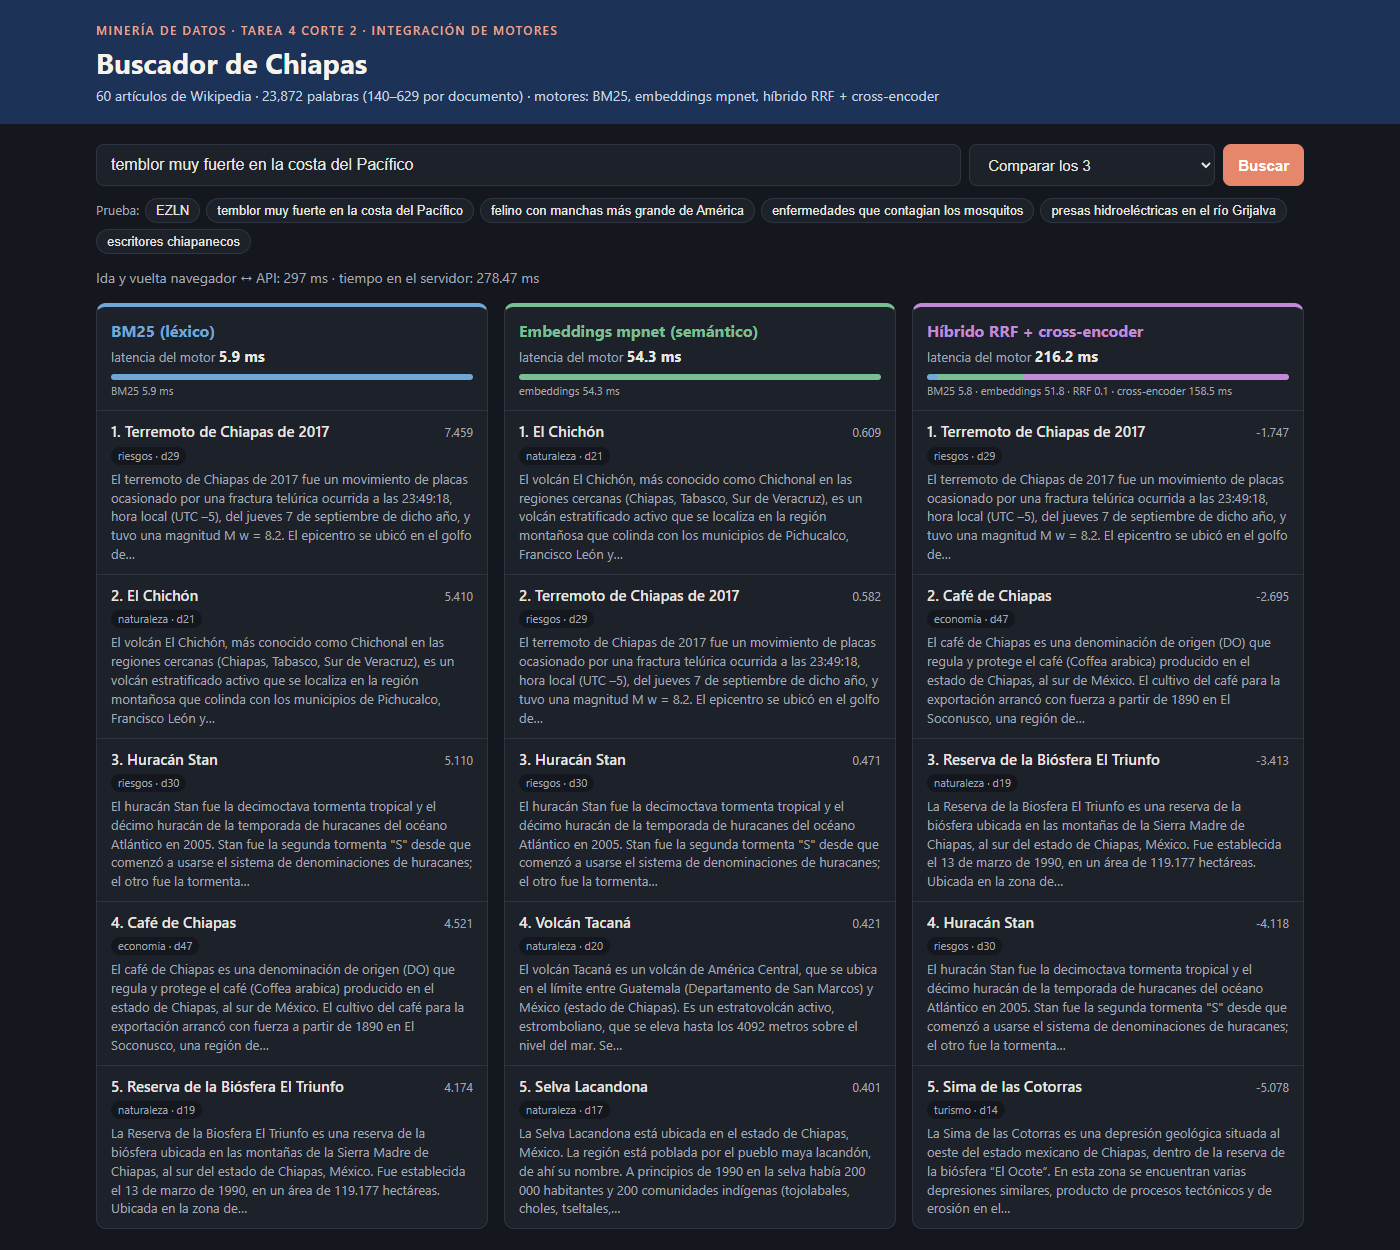
\includegraphics[width=\linewidth]{../figuras/frontend.png}
\caption{Frontend en modo ``comparar los 3'' con la consulta \emph{temblor muy fuerte en la costa del Pacífico}. BM25 y el híbrido ponen el terremoto en primer lugar; los embeddings ponen primero al volcán El Chichón. Los tiempos son de una sola consulta, tomada mientras arrancaba el navegador de la captura; las latencias del reporte salen de la prueba de carga.}
\label{fig:front}
\end{figure}

\paragraph{Entorno.} Windows 11, Python 3.12, NVIDIA RTX 4060 Laptop (8~GB), \term{torch} 2.6 (CUDA 12.4), \term{sentence-transformers} 6.2, \term{spaCy} 3.8, FastAPI 0.115 y Uvicorn 0.34 (1 proceso).

% =====================================================================
\section{Calidad de los resultados}
\label{sec:calidad}

La latencia solo tiene sentido junto con la calidad, así que antes de la prueba de carga se midió qué tan buenos son los resultados. Se escribieron \textbf{19 consultas} con relevancia graduada (3 = el documento trata el tema, 2 = lo trata en parte, 1 = lo menciona), juzgadas leyendo el texto de cada documento (\term{evaluacion/qrels.json}). Se repartieron igual que en el Lab~7:
\begin{itemize}[nosep]
\item \textbf{Léxicas (6):} siglas y nombres propios: \emph{EZLN}, \emph{UNACH}, \emph{Montes Azules}, \emph{Tren Maya}, \emph{Coffea arabica denominación de origen} y \emph{Bonampak y Yaxchilán}.
\item \textbf{Semánticas (6):} paráfrasis que evitan la palabra clave del documento, como \emph{temblor muy fuerte en la costa del Pacífico} (el documento dice \emph{terremoto}), \emph{felino con manchas más grande del continente} (\emph{jaguar}) o \emph{aguardiente artesanal usado en rituales indígenas} (\emph{pox}).
\item \textbf{Mixtas (7):} temas con varios documentos relevantes, como \emph{zonas arqueológicas mayas en la selva} o \emph{presas hidroeléctricas en el río Grijalva}.
\end{itemize}
Se usaron las métricas del Lab~7 (nDCG@5 con ganancia $2^{rel}-1$, MRR y R@5) más P@5. Como ablación se agregó el híbrido \emph{sin} cross-encoder (solo RRF), para separar lo que aporta cada etapa (\term{evaluacion/evaluar\_calidad.py}).

\begin{table}[H]
\centering
\caption{Calidad sobre las 19 consultas. Las tres últimas columnas son el nDCG@5 por tipo de consulta.}
\label{tab:calidad}
\begin{tabular}{lccccccc}
\toprule
Motor & nDCG@5 & MRR & R@5 & P@5 & Léxicas & Semánt. & Mixtas \\
\midrule
BM25 & \textbf{0.922} & \textbf{0.961} & \textbf{0.886} & \textbf{0.379} & \textbf{0.977} & 0.846 & \textbf{0.940} \\
Embeddings (mpnet) & 0.757 & 0.803 & 0.789 & 0.347 & 0.785 & 0.617 & 0.852 \\
\midrule
\textcolor{gris}{Híbrido, solo RRF} & \textcolor{gris}{0.856} & \textcolor{gris}{0.868} & \textcolor{gris}{0.868} & \textcolor{gris}{0.368} & \textcolor{gris}{0.851} & \textcolor{gris}{0.770} & \textcolor{gris}{0.934} \\
Híbrido RRF + cross-encoder & \textbf{0.922} & \textbf{0.961} & 0.838 & 0.358 & 0.963 & \textbf{0.868} & 0.932 \\
\bottomrule
\end{tabular}
\end{table}

\begin{figure}[H]
\centering
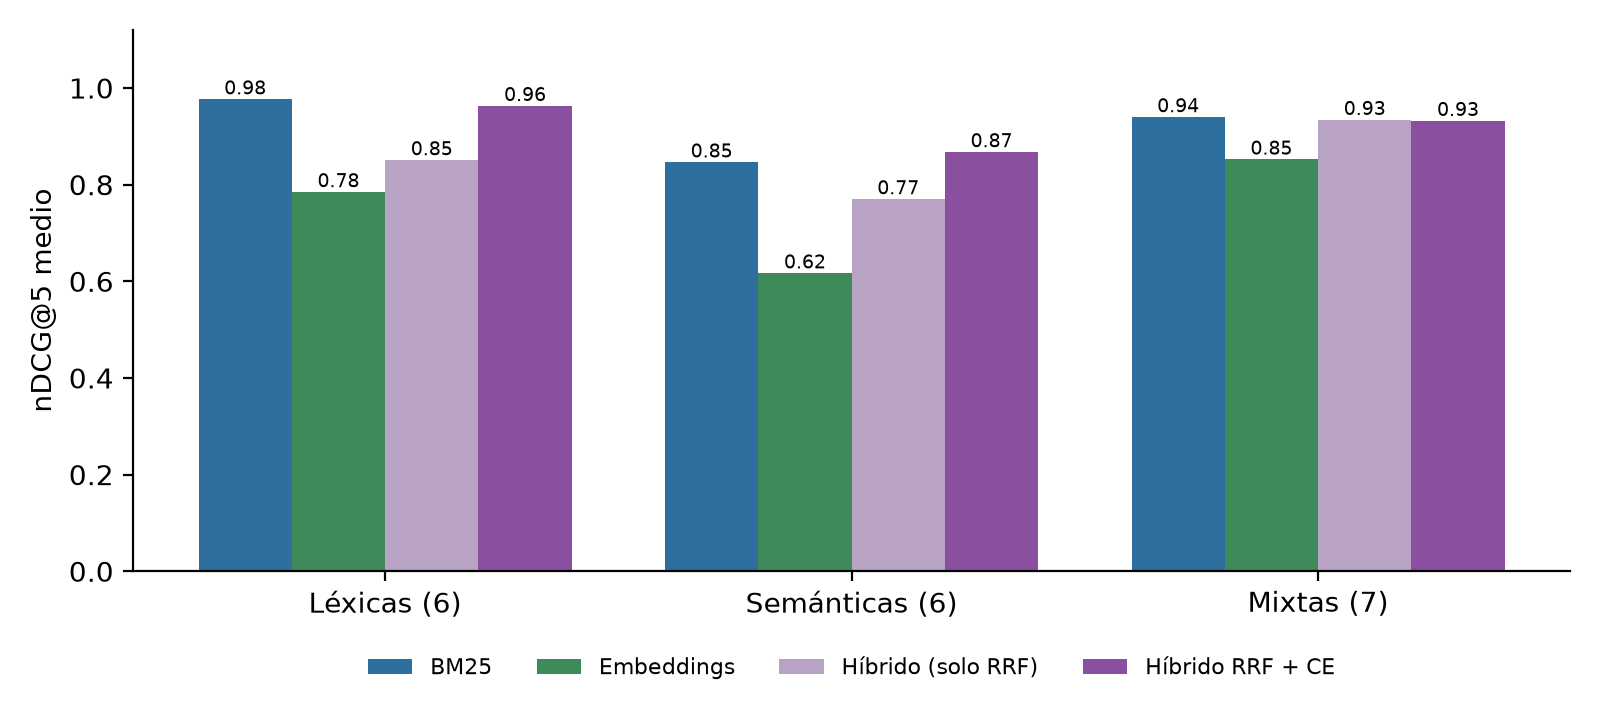
\includegraphics[width=0.85\linewidth]{../figuras/calidad_por_tipo.png}
\caption{nDCG@5 medio por tipo de consulta.}
\label{fig:calidad}
\end{figure}

\textbf{El resultado no es el de la Tarea~3.} Con las 14 notas cortas, BM25 valía 0 en las consultas semánticas y el denso las resolvía todas. En este corpus pasa lo contrario: \textbf{BM25 empata con el híbrido} (nDCG@5 = 0.922) y le saca 0.165 a los embeddings. Las causas son tres:

\begin{enumerate}
\item \textbf{Los documentos largos casi siempre contienen la paráfrasis.} Un artículo de 400 palabras usa muchas palabras para hablar de su tema. Al pasar las consultas ``semánticas'' por el preprocesamiento de BM25, casi todas comparten lemas con su documento relevante: \emph{temblor\ldots} comparte \emph{fuerte}, \emph{costa} y \emph{pacífico} con el artículo del terremoto; \emph{aguardiente\ldots} comparte \emph{aguardiente}, \emph{artesanal}, \emph{ritual} e \emph{indígena} con el del pox; \emph{enfermedades que contagian los mosquitos} comparte \emph{enfermedad} y \emph{mosquito} con el del dengue. En las notas de 40 palabras del Lab~7 esa coincidencia no existía. La única consulta sin vocabulario en común es la del jaguar (solo comparte \emph{continente}), y es justo donde BM25 cae a 0.431.

\item \textbf{Los embeddings encuentran el tema, pero no el documento exacto.} Los errores del denso son documentos ``vecinos'': para \emph{temblor} pone primero \emph{El Chichón} (el volcán, cuyo artículo habla de sismos); para el felino pone primero al cocodrilo; para el ave de plumaje verde pone a la guacamaya antes que al quetzal; para \emph{aguardiente\ldots} devuelve cinco artículos sobre pueblos indígenas y deja fuera al del pox (nDCG = 0). En las léxicas falla con nombres raros: en \emph{Montes Azules} pone primero \emph{Cascadas de Agua Azul} (0.500), y en \emph{Coffea arabica} pone primero \emph{Soconusco} (0.431).

\item \textbf{El encoder lee 128 tokens.} El score de cada documento depende de cómo se parte en pasajes. La ablación (Tabla~\ref{tab:ablacion}) muestra que con el mismo encoder el nDCG@5 va de 0.739 a 0.824 según la representación del documento. Promediar los 2 mejores pasajes o usar el embedding medio rinde más que el máximo que usa el motor. No se cambió el motor porque la variante se elegiría con las mismas 19 consultas con las que se evalúa, que es el mismo sesgo que la Tarea~3 encontró con el $\alpha$ óptimo. Aun la mejor variante (0.824) queda por debajo de BM25.
\end{enumerate}

\begin{table}[H]
\centering
\caption{Ablación del motor denso: cinco formas de representar un documento de 400 palabras con un encoder de 128 tokens (nDCG@5).}
\label{tab:ablacion}
\begin{tabular}{lcccc}
\toprule
Representación del documento & Global & Léxicas & Semánt. & Mixtas \\
\midrule
Máximo sobre pasajes (\textbf{el motor}) & 0.757 & 0.785 & 0.617 & 0.852 \\
Media de los 2 mejores pasajes & \textbf{0.824} & 0.786 & 0.768 & \textbf{0.903} \\
Embedding medio de los pasajes & 0.814 & 0.665 & \textbf{0.902} & 0.867 \\
Solo el primer pasaje (el resumen del artículo) & 0.739 & \textbf{0.818} & 0.650 & 0.748 \\
Documento completo truncado a 128 tokens & 0.739 & \textbf{0.818} & 0.650 & 0.748 \\
\bottomrule
\end{tabular}
\end{table}

\textbf{Qué aporta cada etapa del híbrido.} RRF solo (0.856) queda \emph{entre} los dos motores: arregla lo peor del denso (\emph{aguardiente} pasa de 0 a 0.631 y \emph{Montes Azules} de 0.500 a 0.631), pero cuando el denso mete documentos equivocados en su top-20, RRF los mezcla con los buenos de BM25. El cross-encoder es lo que lo pone a la par de BM25: sube \emph{zonas arqueológicas mayas en la selva} a 0.986 (BM25: 0.759), \emph{aguardiente} y \emph{Coffea arabica} a 1.000, y obtiene el mejor nDCG@5 en las semánticas (0.868). A cambio, baja respecto a RRF en cuatro mixtas (\emph{pueblos indígenas de los Altos}, de 0.884 a 0.752; \emph{bebidas de maíz y cacao}, de 1.000 a 0.947; \emph{escritores chiapanecos}, de 1.000 a 0.920; \emph{ave de plumaje verde}, de 1.000 a 0.983), y ningún sistema resuelve la del jaguar (0.431 en BM25 y en el híbrido).

Con 19 consultas, una diferencia de 0.05 en nDCG equivale a mover uno o dos documentos en una o dos consultas. Las diferencias claras son las grandes: embeddings $\ll$ RRF $<$ BM25 $\approx$ híbrido con cross-encoder.

% =====================================================================
\section{Desempeño: latencia con hasta 50 usuarios concurrentes}
\label{sec:carga}

\subsection{Cómo se midió}

La prueba está en \term{carga/prueba\_carga.py}. Cada \textbf{usuario virtual} es una corrutina de \term{asyncio} que, con \term{httpx}, manda una consulta a \term{/api/buscar}, espera la respuesta y manda la siguiente, sin pausa entre consultas. Es un modelo de carga \emph{cerrado} y es el peor caso: un usuario real tarda unos segundos en leer los resultados. Las consultas se toman al azar de un conjunto de 31 (las 19 de evaluación y 12 más), con semilla fija.
\begin{itemize}[nosep]
\item \textbf{Niveles:} 1, 5, 10, 25 y 50 usuarios concurrentes para cada motor. Cada nivel manda al menos 300 peticiones (500 con 50 usuarios) después de 5 de calentamiento que no se miden. En total fueron \textbf{5\,100 peticiones} en los niveles y 500 en el escenario mixto.
\item \textbf{Escenario mixto:} 50 usuarios en los que cada consulta elige motor al azar. Es lo más parecido al uso real del frontend.
\item \textbf{Latencia:} se mide en el cliente (ida y vuelta HTTP completa) y de ahí salen p50, p95 y p99. También se guarda el tiempo que reporta el servidor en la cabecera \term{X-Tiempo-Servidor-ms}.
\item \textbf{Entorno:} servidor y cliente corren en la misma laptop (sin red de por medio), con Uvicorn en 1 proceso y modelos en la GPU. Las 5\,600 peticiones respondieron \textbf{200 OK}, sin errores.
\end{itemize}

\subsection{Resultados}

\begin{table}[H]
\centering
\caption{Latencia en el cliente (ms) y rendimiento por motor y número de usuarios concurrentes. ``Servidor'' es la mediana del tiempo dentro de FastAPI.}
\label{tab:carga}
\begin{tabular}{llrrrrr}
\toprule
Motor & Usuarios & \textbf{p50} & \textbf{p95} & p99 & Servidor p50 & Peticiones/s \\
\midrule
\multirow{5}{*}{BM25} & 1 & \textbf{11.8} & \textbf{17.0} & 27.3 & 4.3 & 80.3 \\
 & 5 & 25.2 & 30.3 & 41.0 & 16.7 & 193.8 \\
 & 10 & 50.0 & 57.6 & 64.5 & 41.5 & 194.1 \\
 & 25 & 126.4 & 138.9 & 167.7 & 116.7 & 192.5 \\
 & 50 & \textbf{258.5} & \textbf{305.2} & 379.1 & 248.7 & 188.0 \\
\midrule
\multirow{5}{*}{Embeddings} & 1 & \textbf{24.5} & \textbf{35.2} & 40.7 & 16.8 & 38.0 \\
 & 5 & 101.2 & 134.7 & 137.1 & 90.1 & 46.7 \\
 & 10 & 190.9 & 209.9 & 219.5 & 180.1 & 51.8 \\
 & 25 & 490.9 & 595.5 & 606.3 & 478.6 & 48.7 \\
 & 50 & \textbf{957.9} & \textbf{1\,105.9} & 1\,126.0 & 947.6 & 50.3 \\
\midrule
\multirow{5}{*}{Híbrido} & 1 & \textbf{93.2} & \textbf{103.3} & 108.3 & 84.8 & 10.7 \\
 & 5 & 372.8 & 412.5 & 473.5 & 361.7 & 13.2 \\
 & 10 & 742.2 & 787.5 & 809.3 & 730.8 & 13.4 \\
 & 25 & 1\,851.3 & 1\,936.8 & 1\,966.2 & 1\,839.2 & 13.4 \\
 & 50 & \textbf{3\,670.8} & \textbf{3\,742.1} & 3\,754.1 & 3\,659.4 & 13.5 \\
\midrule
Mixto (1/3 cada uno) & 50 & 2\,030.3 & 2\,499.8 & 2\,570.4 & 2\,007.9 & 30.2 \\
\bottomrule
\end{tabular}
\end{table}

\begin{figure}[H]
\centering
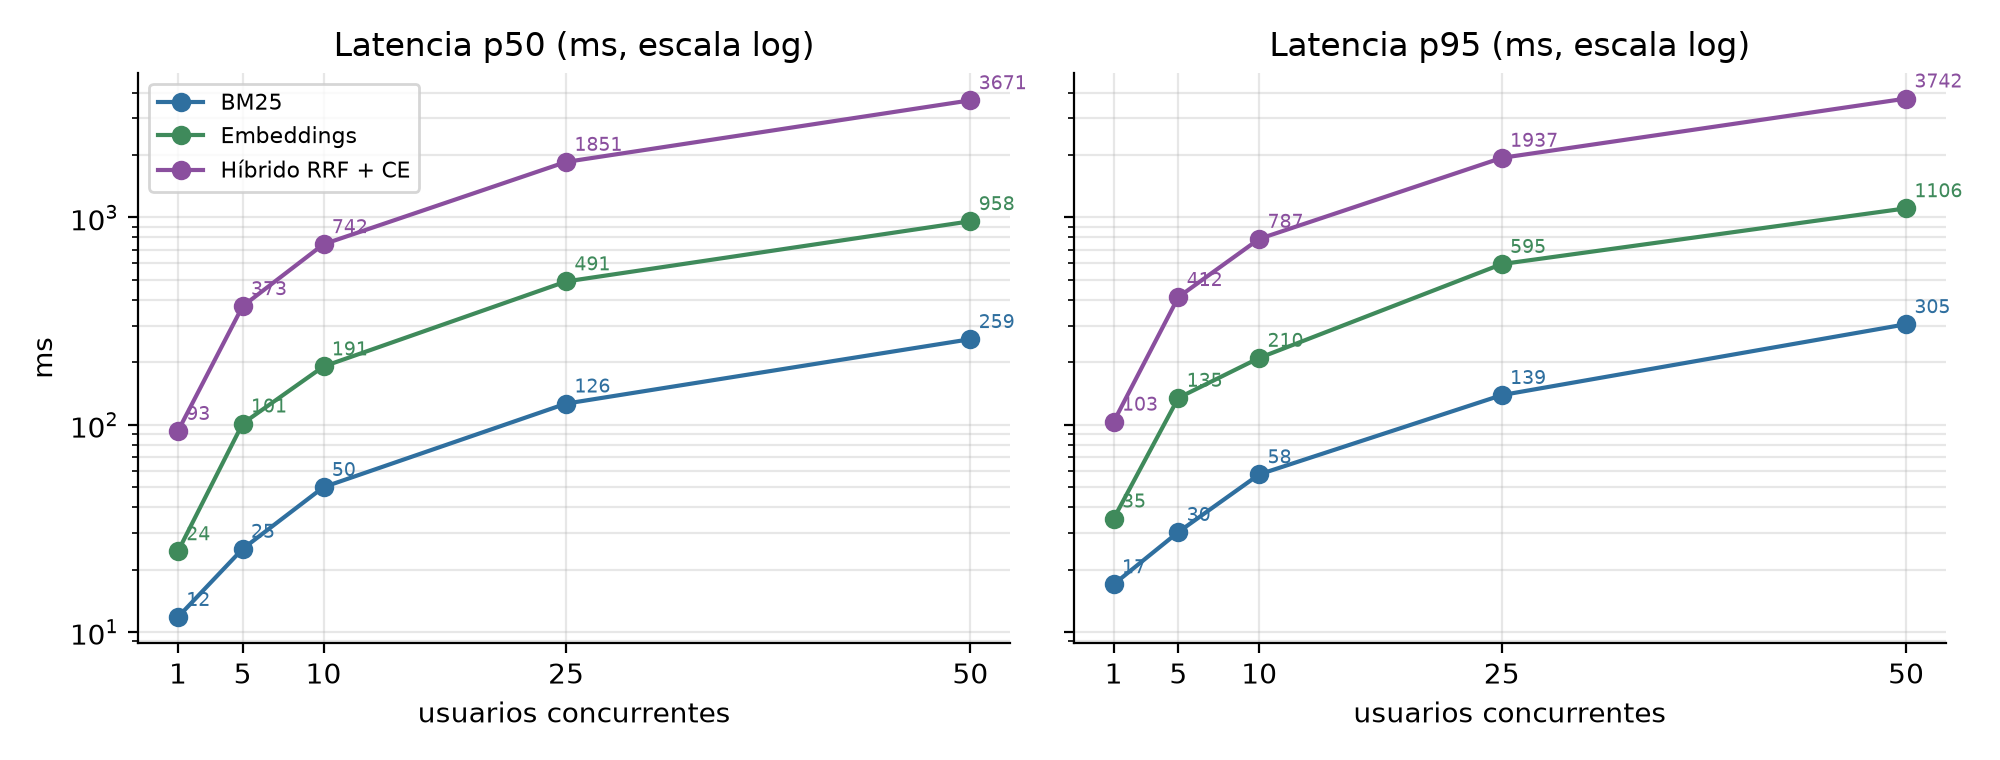
\includegraphics[width=\linewidth]{../figuras/carga_latencia.png}
\caption{p50 y p95 contra usuarios concurrentes (escala logarítmica).}
\label{fig:carga}
\end{figure}

\begin{figure}[H]
\centering
\begin{minipage}{0.47\linewidth}
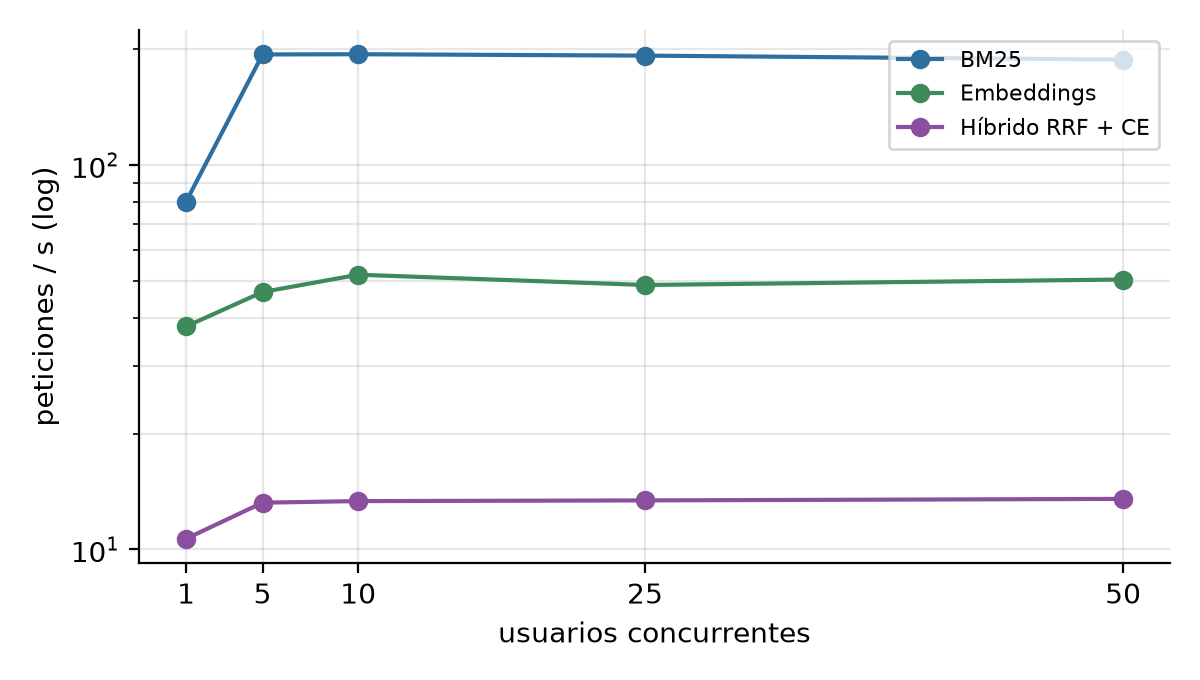
\includegraphics[width=\linewidth]{../figuras/carga_rps.png}
\end{minipage}\hfill
\begin{minipage}{0.52\linewidth}
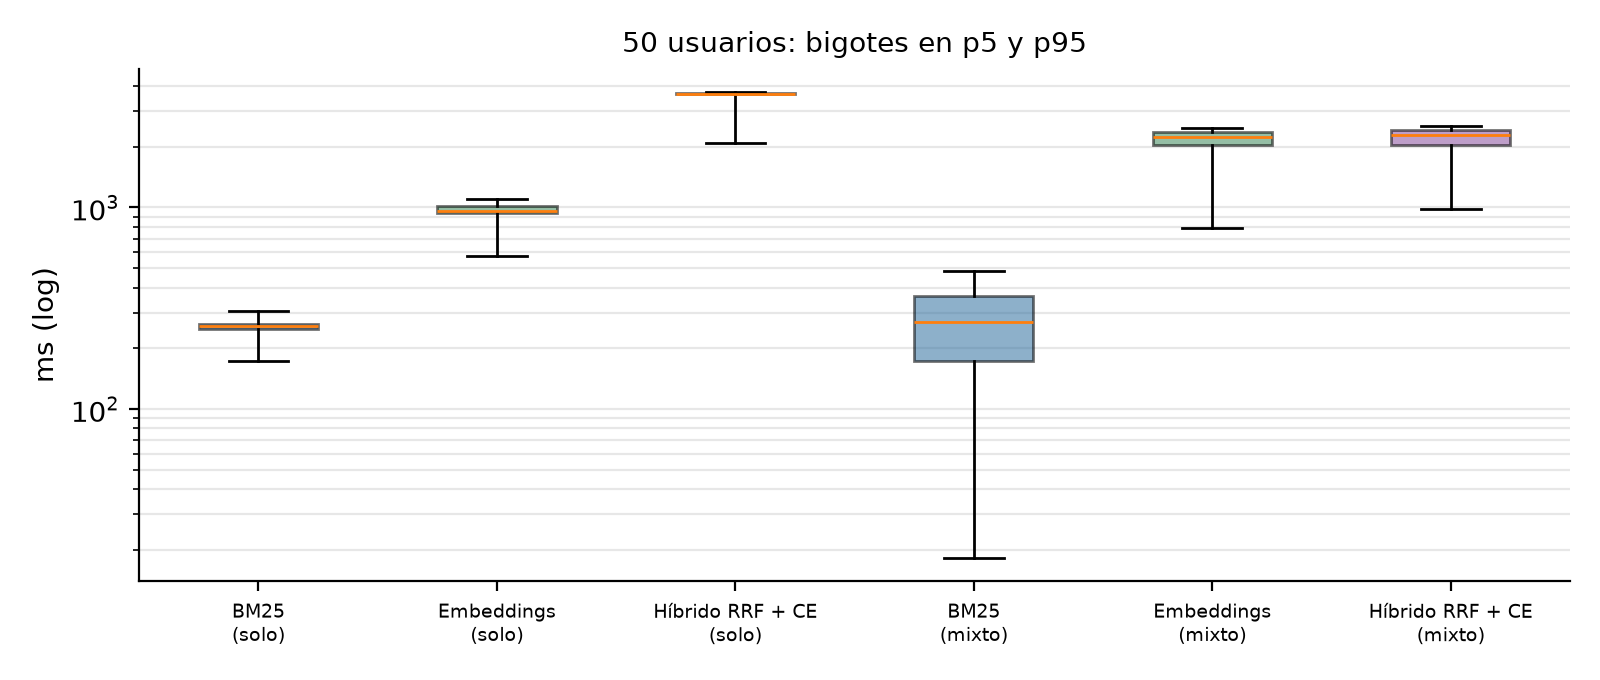
\includegraphics[width=\linewidth]{../figuras/carga_50usuarios.png}
\end{minipage}
\caption{Izquierda: rendimiento (peticiones por segundo). Derecha: distribución de la latencia con 50 usuarios, cada motor solo y en el escenario mixto.}
\label{fig:rps}
\end{figure}

\subsection{Comportamiento de los motores}

\begin{enumerate}
\item \textbf{Con un usuario, el costo sigue el número de modelos.} BM25 tarda 4.3~ms en el servidor, porque solo lematiza la consulta y recorre el índice invertido. Los embeddings tardan 16.8~ms: codifican la consulta en la GPU y hacen un producto matriz--vector de $308 \times 768$. El híbrido tarda 84.8~ms, y más de dos tercios de ese tiempo (60 a 90~ms, según la consulta) se van en el cross-encoder, que lee 10 pares de hasta 512 tokens. Los 7 a 9~ms de diferencia entre cliente y servidor son el costo de HTTP en local.

\item \textbf{Los tres se saturan muy pronto, y después la latencia crece en línea recta.} El rendimiento deja de subir a partir de 5 usuarios: unas \textbf{190 peticiones/s} para BM25, \textbf{50} para los embeddings y \textbf{13.4} para el híbrido. A partir de ahí, agregar usuarios solo alarga la cola, y la latencia sigue la ley de Little ($\text{latencia} \approx \text{usuarios} / \text{rendimiento}$): con 50 usuarios, $50/188 = 266$~ms para BM25 (medido: 259), $50/50.3 = 994$~ms para los embeddings (958) y $50/13.5 = 3.7$~s para el híbrido (3.67~s). Prácticamente todo el tiempo es espera: la mediana dentro del servidor es casi igual a la del cliente.

\item \textbf{La causa es que el servidor procesa una consulta a la vez.} El rendimiento máximo coincide con el inverso del tiempo de una consulta ($1/4.3~\text{ms} \approx 230$, $1/16.8~\text{ms} \approx 60$, $1/84.8~\text{ms} \approx 12$). Es decir, aunque FastAPI tenga 40 hilos, las peticiones avanzan de una en una: BM25 por el GIL de Python y el candado de spaCy, y los otros dos por el candado de la GPU. Se eligió así a propósito, porque usar los modelos desde varios hilos sin candado no es seguro. El precio es que el servidor no escala con la concurrencia.

\item \textbf{p95 queda muy cerca de p50.} Con 50 usuarios, p95/p50 es 1.18 en BM25, 1.15 en embeddings y 1.02 en el híbrido. Como todas las peticiones pasan por la misma cola, la variación entre consultas (consultas más largas, más candidatos) se diluye en el tiempo de espera. La excepción es BM25 con 1 usuario: su p99 (27~ms) es 2.3 veces su p50. Con tiempos tan cortos, cualquier pausa del sistema operativo o de Python pesa mucho (no se investigó la causa exacta).

\item \textbf{En el escenario mixto, el motor lento arrastra a los demás.} Con 50 usuarios repartidos entre los tres motores, BM25 sigue rápido (p50 = 269~ms, p95 = 487~ms), porque usa la CPU y no compite por la GPU. Los embeddings, en cambio, \emph{empeoran} respecto a su escenario solo: p50 de 2\,245~ms contra 958~ms. Las búsquedas densas comparten el encoder con la etapa densa del híbrido, y la GPU se reparte con el cross-encoder, así que quedan formadas detrás de las consultas híbridas. El rendimiento total (30.2 peticiones/s) es el promedio ponderado de los tres.
\end{enumerate}

\textbf{¿Cuántos usuarios aguanta cada motor?} Si se toma como meta un p95 menor a 500~ms (un valor común para que una búsqueda se sienta inmediata), BM25 la cumple con los 50 usuarios (305~ms), los embeddings hasta unos 20 (p95 = 210~ms con 10 y 596~ms con 25) y el híbrido solo hasta unos 5 (413~ms). Con usuarios reales que leen los resultados unos 10~s entre consultas, cada uno manda unas 0.1 consultas por segundo, así que el mismo servidor atendería a unos 1\,900 usuarios con BM25, 500 con embeddings y 130 con el híbrido.

\textbf{Cómo se podría escalar.} Por orden de impacto sobre el cuello de botella, que es la cola de la GPU:
\begin{itemize}[nosep]
\item \textbf{Agrupar consultas} (\emph{dynamic batching}): juntar en un solo lote de GPU las consultas que llegan en una ventana de pocos ms. Codificar 16 consultas cuesta casi lo mismo que codificar una.
\item \textbf{Cache} de las consultas frecuentes (LRU), que en un buscador real se repiten mucho.
\item \textbf{Menos candidatos para el cross-encoder} (5 en lugar de 10) o un cross-encoder más chico o cuantizado (ONNX, int8).
\item \textbf{Varios procesos de Uvicorn} para BM25, que usa la CPU, y separar el motor denso y el híbrido en un servicio de inferencia propio.
\end{itemize}

% =====================================================================
\section{Criterio de decisión}

\subsection{Calidad contra costo}

\begin{table}[H]
\centering
\caption{Los tres motores lado a lado. Latencias medidas en el cliente.}
\label{tab:decision}
\begin{tabular}{lccc}
\toprule
 & BM25 & Embeddings & Híbrido RRF + CE \\
\midrule
nDCG@5 (19 consultas) & \textbf{0.922} & 0.757 & \textbf{0.922} \\
nDCG@5 semánticas & 0.846 & 0.617 & \textbf{0.868} \\
p50 / p95 con 1 usuario (ms) & \textbf{12 / 17} & 25 / 35 & 93 / 103 \\
p50 / p95 con 50 usuarios (ms) & \textbf{259 / 305} & 958 / 1\,106 & 3\,671 / 3\,742 \\
Rendimiento máximo (peticiones/s) & \textbf{$\approx$190} & $\approx$50 & $\approx$13 \\
Usuarios con p95 $<$ 500~ms & \textbf{50+} & $\approx$20 & $\approx$5 \\
Tiempo de arranque & 14~s (spaCy) & 27~s & +4~s sobre los otros dos \\
Necesita GPU & no & recomendable & recomendable \\
Devuelve ``sin resultados'' & sí & no (siempre da $k$) & no \\
\bottomrule
\end{tabular}
\end{table}

\subsection{El criterio}

La elección se hizo en este orden:
\begin{enumerate}
\item \textbf{Calidad mínima aceptable.} Se descarta el motor que se equivoca en el tema. Los embeddings solos quedan fuera en este corpus: su nDCG@5 (0.757) está 0.165 por debajo de los otros dos y fallan en nombres propios (\emph{Montes Azules} $\to$ \emph{Agua Azul}).
\item \textbf{Latencia bajo la carga esperada.} Entre los motores con buena calidad, se elige el que cumple la meta de p95 con la concurrencia esperada. BM25 y el híbrido empatan en nDCG@5, pero BM25 es 8 veces más rápido con un usuario y 14 veces más rápido con 50.
\item \textbf{El tipo de consulta.} El híbrido solo vale lo que cuesta si los usuarios escriben consultas sin el vocabulario del documento. Es el único que mejora en las semánticas (0.868 frente a 0.846 de BM25) y corrige casos que BM25 deja mal, como \emph{zonas arqueológicas mayas en la selva} (0.986 frente a 0.759).
\end{enumerate}

\textbf{Decisión para este sistema:} \textbf{BM25 como motor por omisión} y el \textbf{híbrido como modo ``búsqueda profunda''} que el usuario activa, o que se activa solo cuando BM25 devuelve pocos resultados o scores bajos. Así, casi todas las consultas cuestan 12~ms, y el cross-encoder se usa solo donde puede ayudar. Si hubiera que elegir \emph{un solo} motor para 50 usuarios simultáneos en este hardware, sería BM25: es el único que cumple p95 $<$ 500~ms sin perder calidad. El híbrido sería la mejor opción si el tráfico fuera bajo (menos de 5 usuarios a la vez) o si se le agregara \emph{batching} en la GPU.

\subsection{¿Cuándo usar cada motor según el corpus?}

La comparación con la Tarea~3 muestra que el mejor motor \textbf{depende del corpus}, no solo del algoritmo:

\begin{table}[H]
\centering
\small
\caption{El mismo par de motores en los dos corpus de la unidad.}
\label{tab:corpus2}
\begin{tabularx}{\linewidth}{lXX}
\toprule
 & 14 noticias cortas (Labs 1--7) & 60 artículos de Wikipedia (esta tarea) \\
\midrule
Largo & $\approx$40 palabras & $\approx$400 palabras \\
Vocabulario & breve, una sola forma de decir cada cosa & extenso; repite el tema con sinónimos \\
BM25 nDCG@5 & 0.735 (0 en semánticas) & 0.922 (0.846 en semánticas) \\
Denso nDCG@5 & 0.918 & 0.757 \\
Mejor opción & denso o híbrido & BM25 o híbrido \\
\bottomrule
\end{tabularx}
\end{table}

\begin{itemize}
\item \textbf{BM25} conviene en corpus de \textbf{documentos largos y bien redactados} (enciclopedias, manuales, documentación técnica, expedientes), donde el texto contiene muchas formas de nombrar su tema. También cuando las consultas son \textbf{nombres propios, siglas, códigos o números} (\emph{EZLN}, \emph{Coffea arabica}, un número de expediente), cuando hace falta poder decir ``no hay resultados'' y cuando no hay GPU o se esperan muchos usuarios.
\item \textbf{Los embeddings} convienen en corpus de \textbf{textos cortos} (tuits, títulos, preguntas frecuentes, reseñas, mensajes de soporte), donde la consulta y el documento rara vez comparten palabras. También para buscar entre idiomas (el encoder es multilingüe), para recomendar ``documentos parecidos'' y como primera etapa de un sistema RAG. En documentos largos hay que cuidar el troceo en pasajes, porque el encoder solo lee 128 tokens.
\item \textbf{El híbrido} conviene cuando \textbf{no se sabe de antemano} qué tipo de consulta llegará, o cuando el usuario mezcla nombres con descripciones (\emph{zonas arqueológicas mayas en la selva}), y cuando la precisión del primer resultado importa más que la latencia: búsqueda legal o médica, o el recuperador de un RAG, donde el modelo generativo tarda segundos de todos modos. Su costo crece con el número de candidatos que se re-ordenan, no con el tamaño del corpus.
\end{itemize}

% =====================================================================
\section{Ventajas y desventajas de cada motor}

\subsection*{BM25 (léxico)}
\textbf{Ventajas}
\begin{itemize}[nosep]
\item El más rápido y el que mejor escala: 12~ms con 1 usuario, 259~ms con 50 y unas 190 peticiones/s, sin GPU.
\item Tuvo la mejor calidad global en este corpus (nDCG@5 = 0.922, MRR = 0.961) y es casi perfecto con nombres propios y siglas (0.977).
\item Es explicable: el score se puede descomponer término por término, y en el frontend se ve por qué salió cada documento (palabras resaltadas).
\item Puede responder ``no hay resultados'' (\emph{EZLN} devuelve 1 documento; \emph{UNACH}, 2), en lugar de rellenar con documentos que no tienen que ver.
\item El índice ocupa poco y se actualiza agregando entradas al índice invertido, sin recalcular todo.
\end{itemize}
\textbf{Desventajas}
\begin{itemize}[nosep]
\item Depende de que la consulta y el documento compartan palabras: si no las comparten, falla (\emph{felino con manchas} = 0.431; en las notas cortas de la Tarea~3, 0 en las semánticas).
\item Depende del preprocesamiento: los lemas de spaCy son la mitad del motor, y tardan 14~s en cargar.
\item Coincidencias accidentales: en \emph{temblor\ldots} pone \emph{Café de Chiapas} cuarto porque comparte \emph{costa} y \emph{Pacífico}.
\item Con varios hilos procesa una consulta a la vez (GIL + spaCy); para escalar hay que usar varios procesos.
\end{itemize}

\subsection*{Embeddings mpnet (semántico)}
\textbf{Ventajas}
\begin{itemize}[nosep]
\item Entiende paráfrasis y sinónimos sin listas de sinónimos: en las notas cortas resolvió todas las semánticas, y aquí resuelve \emph{mosquitos} (1.000) y \emph{computadoras que aprenden} (0.860, mejor que BM25 con 0.730).
\item Es multilingüe y no necesita lematizar ni quitar stopwords.
\item Sigue siendo rápido con un usuario (25~ms), y su costo por consulta casi no depende del tamaño del corpus, porque el producto matriz--vector es barato (con millones de documentos se usaría un índice ANN como el HNSW de Qdrant de la Tarea~3).
\end{itemize}
\textbf{Desventajas}
\begin{itemize}[nosep]
\item Fue el peor en este corpus (0.757): encuentra el tema, pero no el documento exacto (volcán en lugar de terremoto, guacamaya en lugar de quetzal, cocodrilo en lugar de jaguar).
\item Falla con nombres propios que no conoce: \emph{Montes Azules} $\to$ \emph{Cascadas de Agua Azul}.
\item Lee solo 128 tokens: con documentos largos hay que partirlos en pasajes, y el resultado cambia hasta 0.085 de nDCG según cómo se haga (Tabla~\ref{tab:ablacion}).
\item Nunca dice ``no hay resultados''. Siempre devuelve $k$ documentos, aunque ninguno tenga que ver.
\item Necesita GPU para escalar, y aun con GPU se satura en unas 50 peticiones/s. En el escenario mixto, su p50 subió a 2.2~s porque comparte la GPU con el híbrido.
\item Es una caja negra: no se puede explicar por qué un coseno de 0.61 le gana a uno de 0.58.
\end{itemize}

\subsection*{Híbrido RRF + cross-encoder}
\textbf{Ventajas}
\begin{itemize}[nosep]
\item Empata con BM25 en calidad global (0.922; MRR = 0.961) y es el mejor en las consultas semánticas (0.868): usa lo mejor de los dos recuperadores.
\item Es el más robusto ante consultas mezcladas: \emph{zonas arqueológicas mayas en la selva} = 0.986 (BM25: 0.759; denso: 0.635).
\item RRF no necesita calibrar escalas ni pesos (la lección de la Tarea~3), y el cross-encoder corrige los errores de la fusión, porque lee la consulta y el documento juntos.
\item El costo del re-ranking depende de cuántos candidatos se reordenan (10), no del tamaño del corpus.
\end{itemize}
\textbf{Desventajas}
\begin{itemize}[nosep]
\item Es el más caro: 93~ms con 1 usuario y 3.7~s con 50; se satura en 13.4 peticiones/s. Solo cumple p95 $<$ 500~ms hasta unos 5 usuarios.
\item Necesita tener cargados tres modelos (spaCy, mpnet y el cross-encoder), con unos 45~s de arranque y $\approx$2.5~GB de memoria de GPU.
\item El cross-encoder no siempre mejora: baja en cuatro consultas mixtas respecto a RRF. Además depende de qué texto se le pase: con el pasaje suelto reordenaba peor que con el documento completo.
\item Hereda las limitaciones de la primera etapa: si el documento relevante no está en el top-20 de BM25 ni en el del denso, el cross-encoder no lo puede rescatar.
\item Es el más difícil de depurar: tiene tres etapas, dos modelos y varios parámetros (profundidad, $k$ de RRF, número de candidatos).
\end{itemize}

% =====================================================================
\section{Conclusiones}

\begin{enumerate}
\item Se integraron los tres motores de la unidad (BM25, embeddings mpnet e híbrido RRF + cross-encoder) en un sistema fullstack: una API REST en FastAPI con la misma interfaz para los tres y un frontend que permite compararlos lado a lado. El corpus son 60 artículos de Wikipedia obtenidos por web scraping (23\,872 palabras, cada documento con al menos 140).
\item \textbf{Calidad:} BM25 y el híbrido empatan (nDCG@5 = 0.922) y los embeddings quedan atrás (0.757). En documentos largos la paráfrasis casi siempre comparte palabras con el texto, y la ventaja del denso que se vio con las notas cortas desaparece. El mejor motor depende del corpus.
\item \textbf{Latencia:} con 1 usuario, p50/p95 = 12/17~ms (BM25), 25/35~ms (embeddings) y 93/103~ms (híbrido). Con 50 usuarios: 259/305~ms, 958/1\,106~ms y 3\,671/3\,742~ms. Las 5\,600 peticiones respondieron sin errores.
\item \textbf{Escalabilidad:} los tres motores se saturan desde los 5 usuarios (190, 50 y 13 peticiones/s), porque el servidor procesa una consulta a la vez (GIL y candado de la GPU). A partir de ahí la latencia crece en línea recta con el número de usuarios, como predice la ley de Little. En carga mixta, el motor más lento retrasa a los que comparten la GPU con él.
\item \textbf{Decisión:} BM25 como motor por omisión y el híbrido como búsqueda profunda opcional. Para escalar el híbrido, lo siguiente sería agrupar consultas en la GPU (\emph{batching}) y guardar en cache las consultas frecuentes.
\end{enumerate}

% =====================================================================
\appendix
\section{Fuentes del corpus}
\label{sec:fuentes}

Los 60 artículos se consultaron en \url{https://es.wikipedia.org} el 5 de noviembre de 2026 (licencia CC BY-SA~4.0). La columna \emph{Rev.} es el identificador de la revisión descargada: la versión exacta se puede abrir con \url{https://es.wikipedia.org/w/index.php?oldid=<Rev.>}.

\makeatletter
{\scriptsize
\setlength{\tabcolsep}{3pt}
\begin{longtable}{@{}l p{4.2cm} l r r p{7.2cm}@{}}
\toprule
ID & Título & Categ. & Pal. & Rev. & URL \\
\midrule
\endhead
\@@input fuentes_tabla.tex
\bottomrule
\end{longtable}
}
\makeatother

\section{Reproducir los resultados}

\begin{lstlisting}
pip install -r requirements.txt && python -m spacy download es_core_news_sm
python scraping/scrape_wikipedia.py          # corpus (ya incluido en data/)
uvicorn app:app --app-dir backend --port 8000 # API + frontend
python evaluacion/evaluar_calidad.py         # tabla de calidad
python evaluacion/ablacion_denso.py          # ablacion del motor denso
python carga/prueba_carga.py                 # prueba de carga (con el servidor arriba)
python carga/graficar_carga.py               # graficas de latencia
\end{lstlisting}

\end{document}
